\documentclass[a4paper,12pt]{article}
\usepackage[hmargin=2cm,top=4cm,headheight=65pt,footskip=45pt]{geometry}
\usepackage[utf8]{inputenc}
\usepackage{graphicx}
\usepackage[hidelinks]{hyperref}
\usepackage{array}
\usepackage{lastpage}
\usepackage{lipsum}
\usepackage{fancyvrb}
\usepackage{color}
\usepackage{fancyhdr}
\usepackage{amsmath}
\usepackage{enumitem}
\usepackage{titlesec}
\usepackage{floatrow}
\usepackage{float}
\usepackage{subcaption}
\usepackage{caption}
\newfloatcommand{capbtabbox}{table}[][\FBwidth]

\definecolor{customGray}{RGB}{128,128,128}
\definecolor{Eblue}{rgb}{0.0, 0.18, 0.39}
%==============Header & Footnote==============

\pagestyle{fancy}
\renewcommand{\headrulewidth}{0pt}
\fancyhead[C,CO,L,LO,R,RO]{}
\fancyhead[C]{%
          \begin{tabular}{|m{3.0cm}|m{10.0cm}|m{2.5cm}|}
          \hline
          \centering\vspace{1.75mm}
\includegraphics[scale=0.275]{logo.pdf} &
          \centering
          {\footnotesize {\sf UNIVERSIDAD EAFIT\\ SCHOOL OF ENGINEERING\\
          \vspace{-1mm}DEPARTMENT OF SYSTEMS AND INFORMATICS}} &
          \centering
          \footnotesize{Page \thepage\ de \pageref{LastPage}\\
          ST245\\
          \vspace{-0.75mm}Data Structures
          }\tabularnewline
          \hline
          \end{tabular}
}
\fancyfoot[C,CO,L,LO,R,RO]{}
\fancyfoot[C]{
          \begin{centering}
            \textcolor{customGray}{{\footnotesize {\sf Professor Mauricio Toro Bermúdez\\
            Phone: $(+57) (4) 261 95 00$ Ext. $9473$. Office: $19 - 627$\\
            \vspace{-1mm}E-mail: mtorobe@eafit.edu.co}}}
        \end{centering}
}

%=============CustomEnumItem===========

\setlist[enumerate]{label=\color{Eblue}\textbf{\roman*.}}

%=============CustomSecSubSec==========

\titleformat{\section}[hang]
{\normalsize\bfseries\itshape\color{black}}{\bfseries\itshape\color{Eblue}\thesection)}{2.5mm}{}

\titleformat{\subsection}[hang]
{\normalsize\bfseries\itshape\color{black}}{\bfseries\color{Eblue}\thesection.\alph{subsection}.}{2.5mm}{}

%==============Title==============

\title{\color{Eblue}\textbf{Laboratory practice No. 4: LinkedList}}
\author{
  \textbf{Juan S. Cárdenas Rodríguez}\\
  Universidad EAFIT\\
  Medellín, Colombia\\
  jscardenar@eafit.edu.co
\and
  \textbf{David Plazas Escudero}\\
  Universidad EAFIT\\
  Medellín, Colombia\\
  dplazas@eafit.edu.co
}

%=============Document=============
\begin{document}
  \maketitle
  \thispagestyle{fancy}

  \section{CODE FOR DELIVERING ON GITHUB}
  The source code can be found in \texttt{Code.py} inside the \texttt{codigo} folder.

  \section{ONLINE EXERCISES}
  The source code can be found in \texttt{Code.py} inside the \texttt{codigo} folder.

  \section{SIMULATION OF PROYECT PRESENTATION QUESTIONS}
    \subsection{Tests}
    You can see the code in \texttt{Code.py} inside the \texttt{codigo}
    folder for further details about each test.
      \begin{figure}[H]
        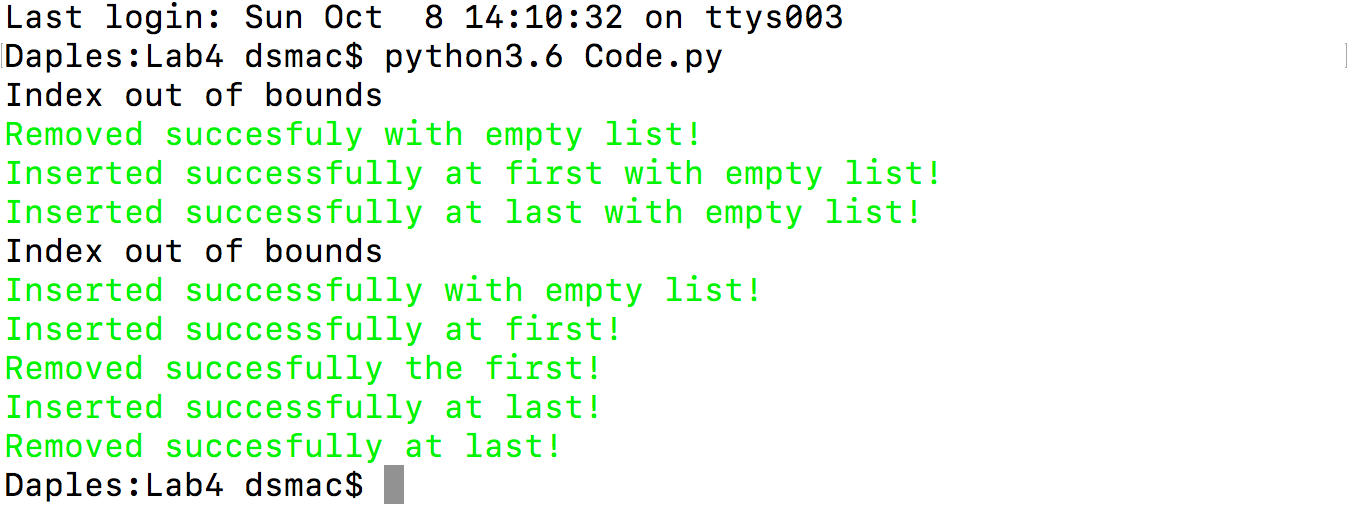
\includegraphics[scale = 0.35]{Tests.png}
        \caption{Tests.}
      \end{figure}
    \subsection{How does exercise 2.1 work?}
    In first place, we recieve the number of blocks that the user wants therefore,
    we create in a loop the linked list so the stack can have the form that the
    user needs. After that, we wait for the user to input a command and, then
    we process it so we know how much is a, b and what operation do we need to do.

    So, in second place, we check if a is equal to b or if they are in the same
    column; if one of this statements is true we just proceed to write the error
    and continue to wait to another instruction. On the other hand, we just make
    the operation he asks us to do. The operations are:
      \begin{itemize}
        \item Move a over b:
      In this operation, we just search for a in all of the stacks that our
      linked list has. To search in the stacks, we just create a temporary
      stack named "stack" and everything that we pop from the original is
      stored in this auxiliar. If we found a, we just pop it ouf the
      temporary stack and, all of the other elements in the data structure,
      we send them to the stack at the index of the linked list that
      corresponds to their number. After that, we just search for b doing
      the same process and, when we find it, we just insert a at the end of
      the stack.

      \item Move a onto b:
      To do this operation, we call the method ``move\_over'' that just makes
      the process described above. And, after that, we just search in the
      linked list till finding b and, removing everything that is in between
      a and b doing a analogous algorithm as the move a over b.

      \item Pile a over b:
      To do this algorithm, we search our list in the same way that we did
      in the operations described below; but, when we found a, we save all
      the numbers that he had on top of him (including a) to another
      auxiliary stack, a\_pile. After that, we just find where b is and
      pile the stacks on top of each other.

      \item Pile a onto b:
      To run this process, we do something like the operation we made on the
      move a onto b. We just call the method ``pile\_over'' and, after that,
      we just erase what is in between a and b.
      \end{itemize}

    \subsection{What's the complexity of exercise 2.1?}
    Exercise 2.1 is $O(n^3)$

  \section{TEST SIMULATION}
    \begin{enumerate}
      \item \begin{itemize}
        \item auxiliar.size()
        \item lista.add(auxiliar.pop())
    \end{itemize}
      \item \begin{itemize}
        \item auxiliar1.size() $>$ 0
        \item auxiliar2.size() $>$ 0
        \item personas.offer(edad)
    \end{itemize}
    \item c) $O(n^2)$
    \end{enumerate}


\end{document}
